\documentclass[crop,tikz]{standalone}
\usetikzlibrary{positioning,arrows,fit,calc}
\pgfdeclarelayer{bg}
\pgfsetlayers{bg,main}
\tikzset{
	>=stealth'
}
\begin{document}
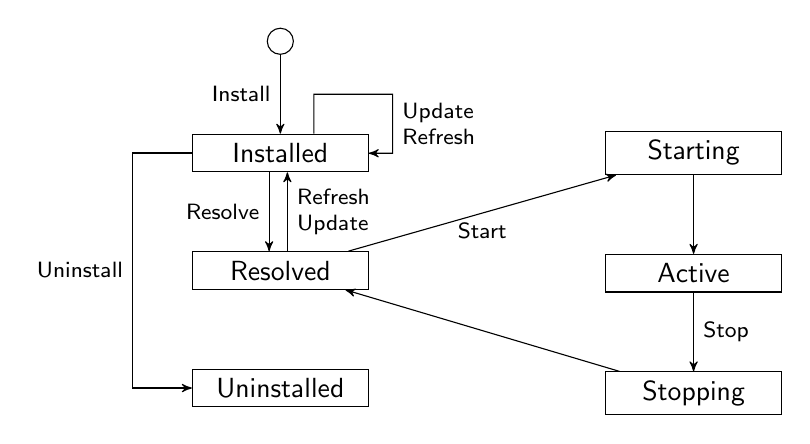
\begin{tikzpicture}[
node distance = 10mm and 30mm,
every node/.style = {
	font = \sffamily
},
state/.style = {
	text width = 2cm,
	draw,
	align = center
},
small/.style = {
	font = \footnotesize\sffamily
}
]

\node[draw, circle] 				(start) 	{};

\node[below=of start, state] 		(installed)	{Installed};
\node[below=of installed, state]	(resolved) 	{Resolved};
\node[below=of resolved, state]		(uninst)	{Uninstalled};

\node[right=of installed, state]	(starting)	{Starting};
\node[below=of starting, state]		(active)	{Active};
\node[below=of active, state]		(stopping)	{Stopping};

\draw[->] (start) -- node[small, left, align=right] {Install} (installed);
\draw[->] (installed.30) -- +(0,0.5) -- + (1,0.5) -- node[small, right, text width= 1cm, align=left] {Update Refresh} +(1,-0.25) -- (installed);
\draw[->] (installed.west) -- +(-.75,0) |- node[small, left, align=right, yshift=1.5cm] {Uninstall} (uninst);
\draw[->] (installed.240) -- node[small, left, align=right] {Resolve} (installed.240 |- resolved.north);
\draw[->] (installed.290 |- resolved.north) -- node[small, right, align=left, text width=1cm] {Refresh Update} (installed.290);
\draw[->] (resolved) -- node[small, below] {Start} (starting);
\draw[->] (starting) -- (active);
\draw[->] (active) -- node[small, right, align=left] {Stop} (stopping);
\draw[->] (stopping) -- (resolved); 
\end{tikzpicture}
	
\end{document}